\section{Implementierung}
Um das ober

\subsection{Unterkapitel 1}\label{Unterkapitel1Link}
Beispiel f�r eine Fu�note\footnote{Fu�noten sind gut.}.

\begin{figure}[htbp]
	\centering
	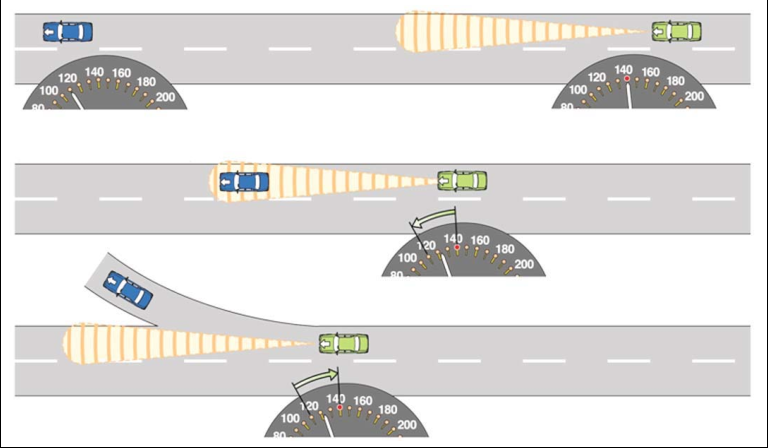
\includegraphics[width=1.0\textwidth]{pics/accBosch.pdf}
	\caption{Folgefahrt Beispielbild}
	\label{fig:accBosch}
\end{figure}

Wie in \ref{Unterkapitel1Link} gezeigt, ist es m�glich, Kapitel zu \citep{Badue2019}verlinken. Abk�rzungen wie das \ac{IfF} werden so dargestellt. Quellen �brigens so \citep{ams09}.

Abbildung ~\ref{fig:accBosch} soll ein Beispielhaftes Bild zeigen.


\subsubsection{Unterunterkapitel1} 

\textbf{\sffamily{M�glichkeit zur weiteren Unterteilung -- Teilkapitel}} Mehr als drei Unterteilungsebenen sollen vermieden werden!
\par
\begingroup
\leftskip=0.8cm
\noindent \textbf{\sffamily{Einger�cktes Teilkapitel}} Derartige Dinge wie einger�ckte Teilkapitel gibt es auch. Falls Du sie brauchen solltest.
\par
\endgroup

\begin{table}[ht]
	\caption{Tabular Umgebung: Simpel formatierte Tabelle}
	\small
	\centering
	\begin{tabular}{ll}
		\toprule
		\multicolumn{2}{c}{Zwei miteinander verbundene Zellen}\\
		\midrule
		Punkt 1 & Adaptive Cruise Control\\
		Punkt 2 & Lane Keeping Assist\\			
		\toprule
		\multicolumn{2}{c}{Schon wieder zwei miteinander verbundene Zellen}\\
		\midrule
		Punkt 3 & Elektronisches Stabilit�tsprogramm\\
		\toprule
	\end{tabular}
	\label{tab:Tabular1}
\end{table}

\begin{table}[ht]
	\caption{Vorteile und Nachteile von Kamera, Radar-, Lidar- und Ultraschallsensor}
	\centering
	\begin{tabular}{|m{0.15\textwidth}<{\centering}|m{0.4\textwidth}<{\centering}|m{0.4\textwidth}<{\centering}|}
		\hline	
		\textbf{Sensor} & \textbf{Vorteile} & \textbf{Nachteile}\\ \hline
		Kamera& 
		\begin{itemize}  
			\setlength\itemsep{0em} 
			\item eine hohe Aufl�sung und Farbskalen �ber das gesamte Sichtfeld haben 
			\item eine farbenfrohe Perspektive der Umgebung bieten 
			\item eine 3D-Geometrie von Objekten bei Stereokameras bereitstellen
			\item kosteng�nstig Im Vergleich zu Lidar sein
		\end{itemize}&
		\begin{itemize}  
			\setlength\itemsep{0em} 
			\item ein leistungsf�higes Berechnungssystem ben�tigen, um n�tzliche Daten zu extrahieren 
			\item empfindlich auf starken Regen, Nebel und Schneefall reagieren 
			\item eine 3D-Geometrie von Objekten bei Stereokameras bereitstellen
			\item begrenzte Reichweite besitzen
		\end{itemize} 
		\\ \hline
		
		Radarsensor& 
		\begin{itemize}  
			\setlength\itemsep{0em} 
			\item lange Strecken bei schlechten Sichtverh�ltnissen vor dem Auto sehen 
			\item klein, leicht und erschwinglich sind 
			\item weniger Strom als ein Lidar-Sensor ben�tigen
			\item im Vergleich zu Lidar robuster gegen Ausf�lle sein
		\end{itemize}&
		\begin{itemize}  
			\setlength\itemsep{0em} 
			\item eine geringe Genauigkeit und Aufl�sung bieten
			\item begrenzte Informationen  (z. B. weder genaue Form- noch Farbinformationen) bekommen
			\item das Problem wegen der gegenseitigen Beeinflussung von Radarsensoren haben
			\item schlechte Azimut- und H�henaufl�sung verf�gen
			\item ohne einer Erh�hung der Leistung Radard�mpfung zeigen
		\end{itemize} 
		\\ \hline
		
		Ultraschall-\newline sensor & 
		\begin{itemize}  
			\setlength\itemsep{0em} 
			\item lange Strecken bei schlechten Sichtverh�ltnissen vor dem Auto sehen 
			\item klein, leicht und erschwinglich sind 
			\item weniger Strom als ein Lidar-Sensor ben�tigen
			\item im Vergleich zu Lidar robuster gegen Ausf�lle sein
		\end{itemize}&
		\begin{itemize}  
			\setlength\itemsep{0em} 
			\item eine geringe Genauigkeit und Aufl�sung bieten
			\item begrenzte Informationen  (z. B. weder genaue Form- noch Farbinformationen) bekommen
			\item das Problem wegen der gegenseitigen Beeinflussung von Radarsensoren haben
			\item schlechte Azimut- und H�henaufl�sung verf�gen
			\item ohne einer Erh�hung der Leistung Radard�mpfung zeigen
		\end{itemize} 
		\\ \hline
	\end{tabular}
\end{table}


\begin{table}[t]
	\caption{Tabular technische Details von Ibeo LUX 8L }
	\centering
	\begin{tabular}{|m{0.4\textwidth}<{\centering}|m{0.6\textwidth}<{\centering}|}
		\hline
		\textbf{Technische Daten} & \textbf{Wert}\\
		\hline
		Reichweite & 50m mit $10\%$ Remission\\
		\hline
		Genauigkeit & 10cm\\
		\hline
		Entfernungsaufl�sung & 4cm\\
		\hline
		Horizontaler �ffnungswinkel & $110^\circ ?50^\circ bis -60^\circ?$ \\
		\hline
		Vertikaler �ffnungswinkel & $6.4^\circ$\\
		\hline
		Horizontale Winkelaufl�sung & $0.25^\circ$\\
		\hline
		Vertikale Winkelaufl�sung & $0.8^\circ$\\
		\hline
		Bildrate & 25.0 Hz\\
		\hline
		Multi-Layer & 8 (2 Paare von 4 Layers)\\
		\hline
		Ausgabe & Roh- und Objektdaten\\
		\hline
		Abma�e (B$\times$T$\times$H) & 164,5$\times$93,2$\times$88mm\\
		\hline
		Gewicht & 998,7g\\
		\hline
	\end{tabular}
	\end{table}
	
\subsubsection{Das zu verwendendes Sensormodell}
\begin{table}[h]
	\caption{Tabular Umgebung: Etwas komplexere Tabelle}
	\centering
	\begin{tabular}{|c|c|c|c|c|c|c|c|c|c|}
		\cline{2-10}
		\multicolumn{1}{c|}{} & \rotatebox{90}{Fahrzeug-CAN} & \rotatebox{90}{GPS-System} & \rotatebox{90}{ESP-Cluster} & \rotatebox{90}{Correvit} & \rotatebox{90}{Lichtschranke} & \rotatebox{90}{Radar} & \rotatebox{90}{Lidar} & \rotatebox{90}{Kreiselplattform} & \rotatebox{90}{Webcam, Leuchtdiode} \\
		\hline
		\multicolumn{10}{|c|}{}  \\
		\multicolumn{1}{|c}{\bfseries{Subjekt}} & \multicolumn{9}{c|}{}  \\
		\hline
		\hline	
		\multicolumn{1}{|c|}{Setzgeschwindigkeit}  &  &  &  &  &  &&  &  & x\\		
		\hline	
		\multicolumn{10}{|c|}{}  \\
		\multicolumn{1}{|c}{\bfseries{relative Gr��en}} & \multicolumn{9}{c|}{}  \\
		\hline
		\multicolumn{1}{|c|}{Triggersignal}  &  & x &   &  & x &   &  & & x \\		
		\hline	
		\multicolumn{10}{|c|}{}  \\
		\multicolumn{1}{|c}{\bfseries{Objekt}} & \multicolumn{9}{c|}{}  \\
		\hline
		\multicolumn{1}{|c|}{L�ngsgeschwindigkeit} & x  & x &  & x &   &  &&   &    \\	
		\hline
	\end{tabular}
	\label{tab:sensorik}
\end{table}

Nachfolgend das Beispiel f�r eine Aufz�hlung mit Itemize.
\begin{itemize}
	\item Reaktionszeit $\mathrm{\Delta t_{react}}$
	\item Im oberen Punkt sieht man auch sch�n die Einbindung von Formeln in den Text.
\end{itemize}

$v_{Obj.}$ = 120\,km/h \\
Einheiten sollten nicht kursiv dargestellt werden und werden vom Zahlenwert durch ein schmales Leerzeichen (Backslash und Komma) getrennt.

Es gibt eine Vielzahl von Gleichungsumgebungen. Equation ist eine davon. Die Gleichung ergibt nat�rlich keinen tieferen Sinn:
\begin{equation}
	x_{obj} = \frac{s^{2} \cdot a \cdot \sqrt{b}}{234 \cdot h_{ego}}
\end{equation}

